\documentclass[%
 letter,
%superscriptaddress,
%groupedaddress,
%unsortedaddress,
%runinaddress,
%frontmatterverbose, 
%preprint,
%preprintnumbers,
%nofootinbib,
%nobibnotes,
%bibnotes,
 amsmath,amssymb,
%prb,
%rmp,
%prstab,
%prstper,
%floatfix,
]{revtex4-2}
\usepackage{soul}
\usepackage{graphicx}% Include figure files
\usepackage{dcolumn}% Align table columns on decimal point
\usepackage{bm}% bold math
\usepackage{xcolor}% 
% \usepackage{luacolor,lua-ul} %for usage of style attributes - background color

\newcommand{\hly}[1]{\colorbox{lime}{\parbox{\columnwidth}{#1}}}

%\usepackage{hyperref}% add hypertext capabilities
%\usepackage[mathlines]{lineno}% Enable numbering of text and display math
%\linenumbers\relax % Commence numbering lines

%\usepackage[showframe,%Uncomment any one of the following lines to test 
%%scale=0.7, marginratio={1:1, 2:3}, ignoreall,% default settings
%%text={7in,10in},centering,
%%margin=1.5in,
%%total={6.5in,8.75in}, top=1.2in, left=0.9in, includefoot,
%%height=10in,a5paper,hmargin={3cm,0.8in},
%]{geometry}
\newcommand{\highlightmath}[1]{\colorbox{lime}{$\displaystyle #1$}}

\newcommand\tmu{\tilde{\mu}}

\newcommand\eps{\varepsilon}
\renewcommand\L {\mathcal{L}}

% \renewcommand{\citet}[1]{ref.~\cite{#1}}
% \renewcommand{\Citet}[1]{Ref.~\cite{#1}}
\newcommand{\citets}[1]{refs.~\cite{#1}}
\newcommand{\Citets}[1]{Refs.~\cite{#1}}
\newcommand{\davg}[1]{\langle {#1} \rangle}
\newcommand{\n}{\\ \nonumber \\ }
\newcommand{\nn}{\nonumber}
\newcommand{\nnn}{\\ \nonumber \\ \nonumber}

\newcommand\ie{\textit{i.e.},~}
\newcommand\eg{\textit{e.g.},~}
\newcommand{\omicron}{o}

\newcommand{\pd}[1]{\partial_{#1}}
\renewcommand{\vec}[1]{\boldsymbol{#1}}
% \renewcommand{\bs}[1]{\boldsymbol{#1}}
\newcommand{\M}[1]{\mathbf{#1}}
\newcommand{\grad}{\nabla}
\newcommand{\cross}{\vec{\times}}
\newcommand{\laplacian}{\nabla^2}
\newcommand{\J}{\mathcal{J}}
\newcommand{\Ju}{\mathcal{J}^{\vec{u}}}
\newcommand{\Jw}{\mathcal{J}^{\omega}}

\newcommand{\Juo}{\mathcal{J}^{u}_0}
\newcommand{\Juf}{\mathcal{J}^{u}_f}
\newcommand{\JUo}{\mathcal{J}^{\vec{u}}_0}
\newcommand{\JUf}{\mathcal{J}^{\vec{u}}_f}
\newcommand{\Jwo}{\mathcal{J}^{\omega}_0}
\newcommand{\Jwf}{\mathcal{J}^{\omega}_f}

\newcommand{\sump}[2]{\sideset{}{'}\sum_{{#1}=0}^{#2}}

\newcommand{\eq}[1]{(\ref{#1})}
\newcommand{\eqs}[2]{(\ref{#1})~\&~(\ref{#2})}
\newcommand{\eqss}[2]{(\ref{#1})--(\ref{#2})}

\newcommand{\Eq}[1]{Eq.~(\ref{#1})}
\newcommand{\Eqs}[2]{Eqs.~(\ref{#1})~\&~(\ref{#2})}
\newcommand{\Eqss}[2]{Eqs.~(\ref{#1})--(\ref{#2})}

\newcommand{\fig}[1]{Fig.~(\ref{#1})}
\newcommand{\figs}[2]{Figs.~(\ref{#1})~\&~(\ref{#2})}
\newcommand{\T}{{\cal T}}
\newcommand{\Z}{{\cal Z}}

\newcommand{\xbar}{\ensuremath{\overline{X}}}
\newcommand{\mJ}{\ensuremath{\mathcal{J}}}



\begin{document}
\section*{Report of the First Referee -- EM12134/O'Connor}
  
This paper presents three methods for solving inverse problems DAL, SBI, and QRM. The paper is very well written, with a thorough introduction and a clear presentation of the methods and results. While I am generally in favor of this paper being accepted, I have some comments I would like to see addressed first.  

\begin{enumerate}

\color{black}\item In the introduction it is said that '…-chi(x,0) which constitutes  the gradient or functional derivative of…'. This is true for how you  have defined the Lagrangian, but is not necessarily the case in  general. For example, a sign change of the adjoint variable in the  Lagrangian would change the sign here so that the gradient would be +  chi(x,0). Could this be rephrased to be more general until you define the Lagrangian.  \\
\color{blue}\begin{itemize}

\item Section I, edit: "Backward integration of the adjoint equations allows us to compute the gradient or functional derivative"
  
\end{itemize}\color{black}\item In the introduction it is said that DALs shortcomings are due to  'missing terms'. I'm not sure of this phrasing. Maybe it is the cost  functional that is the issue, as you show in section 5.  \\
\color{blue}\begin{itemize}

\item We rewrote this paragraph, see our reply to item 3. Instead saying that DALs shortcomings are due to 'missing terms', we claim that DALs shortcomings can be alleviated by appending the adjoint with extra terms.
\item We have updated every instance of the phrase "missing terms" --> "additional terms" or "additional advective terms".


\end{itemize}\color{black}\item You also say that the issues you encounter with DAL would not be  fixed by using a discrete adjoint. This is not demonstrated in the  paper. I agree that the formulation would be the same with regards to  the 'missing terms' and analysis of section 5. However, might the  issues with DAL encountered in this paper potentially stem from an  incorrect gradient being calculated due to discretization errors from  the continuous adjoint formulation?  \\
\color{blue}\begin{itemize}

\item We rewrote this paragraph as follows: "In practice, researchers often customize the DAL algorithm to improve performance in specific cases. For example, [15] used the conjugate-gradient method with a discrete adjoint formulation to optimize initial conditions subject to norm constraints. For the PNS inverse problem, [9] combined Principle Orthogonal Decomposition (POD) with four-dimensional variational assimilation (4DVAR), an optimal control technique analogous to DAL. In both examples, researchers reduced the computational cost of each DAL iteration by reformulating the adjoint while simultaneously reducing the required number of DAL iterations by implementing Quasi-Newton minimization routines. For this investigation, we take a different approach. Instead of reformulating the adjoint or changing the way in which gradient information is used, we will later demonstrate that DAL's shortcomings in the context of Navier--Stokes inversion can be mitigated by appending the adjoint system with additional advective terms."

\end{itemize}\color{black}\item No verification of the adjoint method is given, so readers cannot  be sure of how accurate the gradient is. Perhaps you could add a  verification of the gradient in a specific direction returned by the  adjoint for a short time horizon T where it should be reasonably  accurate for a continuous formulation. \\
\color{blue}\begin{itemize}

\item Evaluating the accuracy of gradients in high-dimensional spaces is challenging. In our 1D KdV-Burgers example problem, we can approximate the gradient of $\mathcal{J}^u_f$ using the \texttt{scipy.optimize.approx\_fprime} function, which relies on the finite difference approximation. We must choose a point in the space of initial conditions to compare gradients. For this, we use the simple backward integration (SBI) initial guess which is described in section III as well as the appendix. We find that the adjoint-obtained gradient has a relative $L_2$ error $<$ 1e-3 and absolute $L_2$ error $<$ 2e-4. Their magnitudes have a ratio $\sim$ 1.00005 and the dot product (projection) of the normalized gradients $\sim$ 0.9999995.
\item For the 2D Navier--Stokes experiment, we again compute the gradient of $\mathcal{J}^{\mathbf{u}}_f$ using the \\ \texttt{scipy.optimize.approx\_fprime} method. To reduce the computational cost of this task, we changed the following parameters: $t_f=5$, $Nx \times Nz = 32 \times 64$, $\Delta t = 0.005$, $\rm{Re}\equiv \nu^{-1} = 5,000$. We use the SBI initial guess as the point at which to compare gradients. In this case, the relative $L_2$ error $<$ 1e-2, absolute $L_2$ error $<$ 1e-4. Their magnitudes have a ratio $\sim$ 0.999994 and the dot product (projection) of the normalized gradients $\sim$ 0.999995.

\item In section III, we appended: "We verify the adjoint solver's accuracy by comparing its output to a gradient obtained via finite-difference."
\item In section IVA, we appended: "We verify the accuracy of the adjoint solver by using the finite-difference approximation to reproduce the gradient at low-resolution."

\end{itemize}\color{black}\item At the end of section 2A it  is said that adjoints require storing the forward solve in memory. Is this not also the case for SBI and QRM? So this is a potential area of  improvement for all the methods presented?  \\
\color{blue}\begin{itemize}
  
  \item Yes this is true. We removed these two sentences because they are somewhat redundant. In the second paragraph of section III, we already state: "While computing $u(x, t)$, we store the solution vector at each timestep."
  
\end{itemize}\color{black}\item In section 3, figure 4, I am a bit confused by the DAL results. It  appears that the LB and GD approaches converge rather poorly. This may  be the case, but my main issue is that there are places where the cost  functional increases rather than decreases. In most gradient descent  algorithms (such as those in scipy.optimize.minimize) this can never  happen. At each iteration a line search is done to ensure that the  cost functional decreases at every iteration. Is that the case for  your approach? If so why are there increases in figure 4? In my  experience line searches are critical in order to ensure fast  convergence.  \\
\color{blue}\begin{itemize}
  
  \begin{figure}[h]
    \centering
    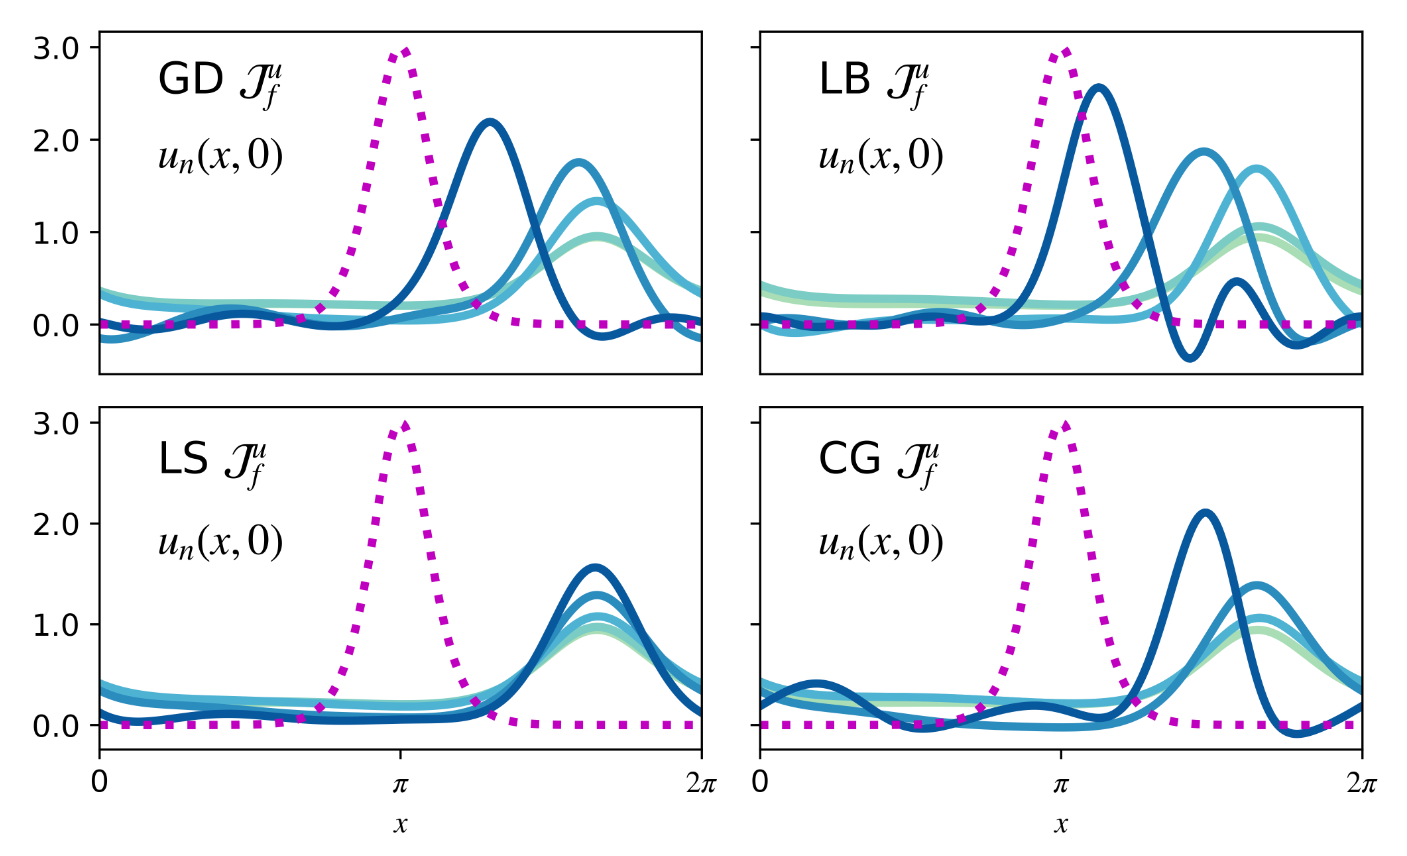
\includegraphics[width=5in]{Pasted image 20240221182636.png}
    \caption{}
  \end{figure}
   
\item Exact line searches require several evaluations of the objective functional. In our case, each evaluation necessitates its own simulation. We did experiment with using the \texttt{scipy.optimize.line\_search} method, which has some compatible features:
	1. This is an inexact line search. Each evaluation of the objective functional is accompanied by a gradient evaluation, such that we utilize the forward and backward solves of the adjoint loop.
	2. \texttt{line\_search} can be used with any descent direction. We use the (negative) gradient for simplicity.
\item L-BFGS performs significantly better than every other \texttt{scipy.optimize} routine (using the default parameters), including \texttt{scipy.optimize.line\_search}
\item The intermittent increases or "spikes" in the final error ($\mathcal{J}_f^u$) are due to the scipy's L-BFGS method. This is a quasi-newton method which evaluates the gradient and the objective at several points prior to taking a descent step. In other words, we were showing the errors at intermediate steps in the optimization routine, because we want compare each method based on the number of solves (forward and backward).
\item In the updated manuscript, we filtered out these intermittent spikes so that the final error ($\mathcal{J}_f^u$) decreases monotonically.
\item In Figure 1 of this report, we plot the trial initial conditions for the KdVB inverse problem for four DAL cases: gradient descent (top left), L-BFGS (top right), line\_search (bottom left), and conjugate-gradient (bottom right). This figure is not included in the manuscript, but the top two panels are identical to those in Figure 11. The primary issue we face with this class of inverse problems is that their gradients rapidly change direction in the space of initial conditions. Line searches do not appear to mitigate this problem.

\end{itemize}\color{black}\item In section 4A equation (16) there is a missing term in your adjoint  equation of the form $-\mu \cdot (\nabla u)^T$ which is present in your  reference [28]. Is this a typo?  \\
\color{blue}\begin{itemize}
  
  \item This was a typo. Thank you for your diligence.

\end{itemize}\color{black}\item Again, in figures 8 and 9 can you clarify why the DAL approaches  have increases in the cost functional?  \\
\color{blue}\begin{itemize}
  
\item We addressed this concern in our reply to item 6 and updated these figures.

\end{itemize}\color{black}\item Section 5 is very interesting. It appears to me that it can be  interpreted from this that QRM and SBI are forms of DAL, but where the  adjoint equation is regularized either through changing the sign of  the diffusion term or through hyperdiffusion. Is this the case?  \\
\color{blue}\begin{itemize}

\item The QRM backward integration equations are indeed regularized adjoint systems. We appended the following text to Section V: "As $\varepsilon\to 0$, QRM backward integration approaches the ill-posed nonlinear adjoint which minimizes $\mathcal{J}^u_0$. From this perspective, QRM is a regularized form of DAL."
\item Referring to SBI as a "form of DAL" might invoke controversy from the optimal control community. Instead, we point out the resemblance between SBI and DAL in the following ways:

	1. Section II, Fig. 1, Caption: "Simple Backward Integration (SBI) is a hybrid method, which supplements the linear DAL system with two additional advective terms."

	2. Section IV, "SBI backward integration combines the linear adjoint which minimizes $\mathcal{J}^u_f$ with the additional terms appearing in the ill-posed nonlinear adjoint"

\end{itemize}\color{black}\item The cost functional given by (22) is also interesting as  calculating it is ill-posed since it requires integrating the direct  equations backwards in time. Does this explain why in the SBI and QRM  approaches you get an approximate gradient, but no value of the cost  functional which could otherwise be used for gradient descent  algorithms?  \\
\color{blue}\begin{itemize}

\item We do (briefly) point this out in Equation 3 and the accompanying text in the introduction.
\item Section V illustrates the relationship between SBI/QRM and the inaccessible cost functional $\mathcal{J}_0^u$. Earlier, in Section II,  we introduce SBI/QRM as methods which approximate the initial deviation $u'(x,0)$ even though this is equivalent to approximating the gradient of $\mathcal{J}_0^u$. We believe that this particular ordering of topics makes the paper easier to interpret.

\end{itemize}\color{black}\item Section 5 also shows that the missing terms in the DAL approach  are actually forcing terms to the adjoint equations stemming from a  cost functional with an integral-in-time component. This links to my  previous comment that 'missing terms' may not be the correct term.  They seem more like extra terms that account for the different cost  functional used.  \\
\color{blue}\begin{itemize}

\item We have updated every instance of the phrase "missing terms" --> "additional terms" or "additional advective terms".

\end{itemize}\color{black}\item In general throughout the paper as all of the approaches are gradient based, could local minimums be found?  \\
\color{blue}\begin{itemize}
  
\item The gradient-based algorithms we tested (L-BFGS, gradient-descent w/ Barzilai--Borwein step sizes, line search, conjugate-gradient) are all guaranteed to converge to a local minimum, eventually.
\item We state this explicitly in Section VIA: "This gradient can be used to refine the trial initial condition toward a local extremum. However, the number of iterations required to approximate said extremum depends on the user's initial guess."
\item Although local minima can be found in theory, in practice this is difficult because of the problems' ill-conditioning. We tried running the DAL cases for several thousand iterations (not shown in the manuscript). Despite this we were unable to confidently identify local extrema.
  
\end{itemize}\color{black}\item Again in figure 11, 12 and 13 there are increases in the cost functional with the DAL method.  \\
\color{blue}\begin{itemize}
  
\item We addressed this concern in our reply to item 6 and updated these figures.

\end{itemize}\color{black}\item By no means an essential comment to address, but would you  consider making the numerical code used for this paper available so  that readers can easily try out these methods for themselves?  \\
\color{blue}\begin{itemize}

\item Section III, we appended: "Our code for this paper is available at https://github.com/liamoconnor9/adjop"
\end{itemize}
\end{enumerate}
\end{document}